\section{Descrizione del firmware PX4 Autopilot}
Il firmware utilizzato nelle simulazioni di software in the loop e processor in the loop è il PX4 Autopilot \cite{px4Firmware}, \cite{px4Guide}.
	
Questo software mette a disposizione diverse funzionalità per avere un sistema di gestione e controllo robusto e affidabile, implementato in diversi tipi di sistemi. L'implementazione non è quindi specifica solo a mezzi aerei di qualsiasi configurazione, ma anche a velicoli di terra, marini e razzi. Il software è open-source e vanta del contributo di parecchi sviluppatori, dagli esperti del settore a contributi di livello accademico. Lo sviluppo open-source permette quindi di aggiungere o modificare le funzionalità messe a disposizione in modo da soddisfare le proprie esigenze e arricchire il progetto generico di nuove funzionalità utili ad altri. Il sistema operativo sulla quale viene eseguito materialmente il codice può essere Nuttx o Linux/MacOS la cui distinzione principale in questa applicazione è solo nella gestione di task e thread.

Il sistema operativo Nuttx è un sistema RTOS (Real-Time Operating System) è svilupato appositamente per implementazioni embedeed. Essendo sviluppato per un contesto specifico ha tutte le caratteristiche necessarie per essere eseguito in sistemi che devono avere prestazioni migliori con poche risorse disponibili. Vengono utilizzati gli standard POSIX e ANSI \cite{Nuttx}. Inoltre, sono implementate funzionalità di programmazione concorrenziale per l'esecuzione di processi in parallelo. Le funzionalità del firmware vengono eseguite in questo sistema come task separati e ogni task può eseguire diversi thread.
Nell'implementazione su sistemi Linux/MacOS invece i moduli sono eseguiti come thread del processo principale, non c'è quindi una distinzione tra threads e tasks, oltre a non essere ottimizzato per sistemi embedeed.


\subsection{Architettura del software}
Il firmware è principalmente suddiviso in due categorie di moduli:
\begin{itemize}
	\item \textbf{Flight stack} : composta dalla parte che stima lo stato del sistema e il relativo controllo
	\item \textbf{Middleware} : composta dalle interfacce che collegano i vari moduli interni di PX4 tra di loro e verso l'esterno, con la possibilità di integrare gli hardware utilizzati.
\end{itemize}

Il sistema quindi separa le varie funzionalità in moduli separati, eseguiti in modo indipendente che scambiano i dati e comandi tra di loro e con l'esterno attraverso messaggi asincroni.
Nella figura \ref{fig:px4.architettura} è riportato lo schema di alto livello del software di PX4 e la sua modularità.

\begin{figure}
	\centering
	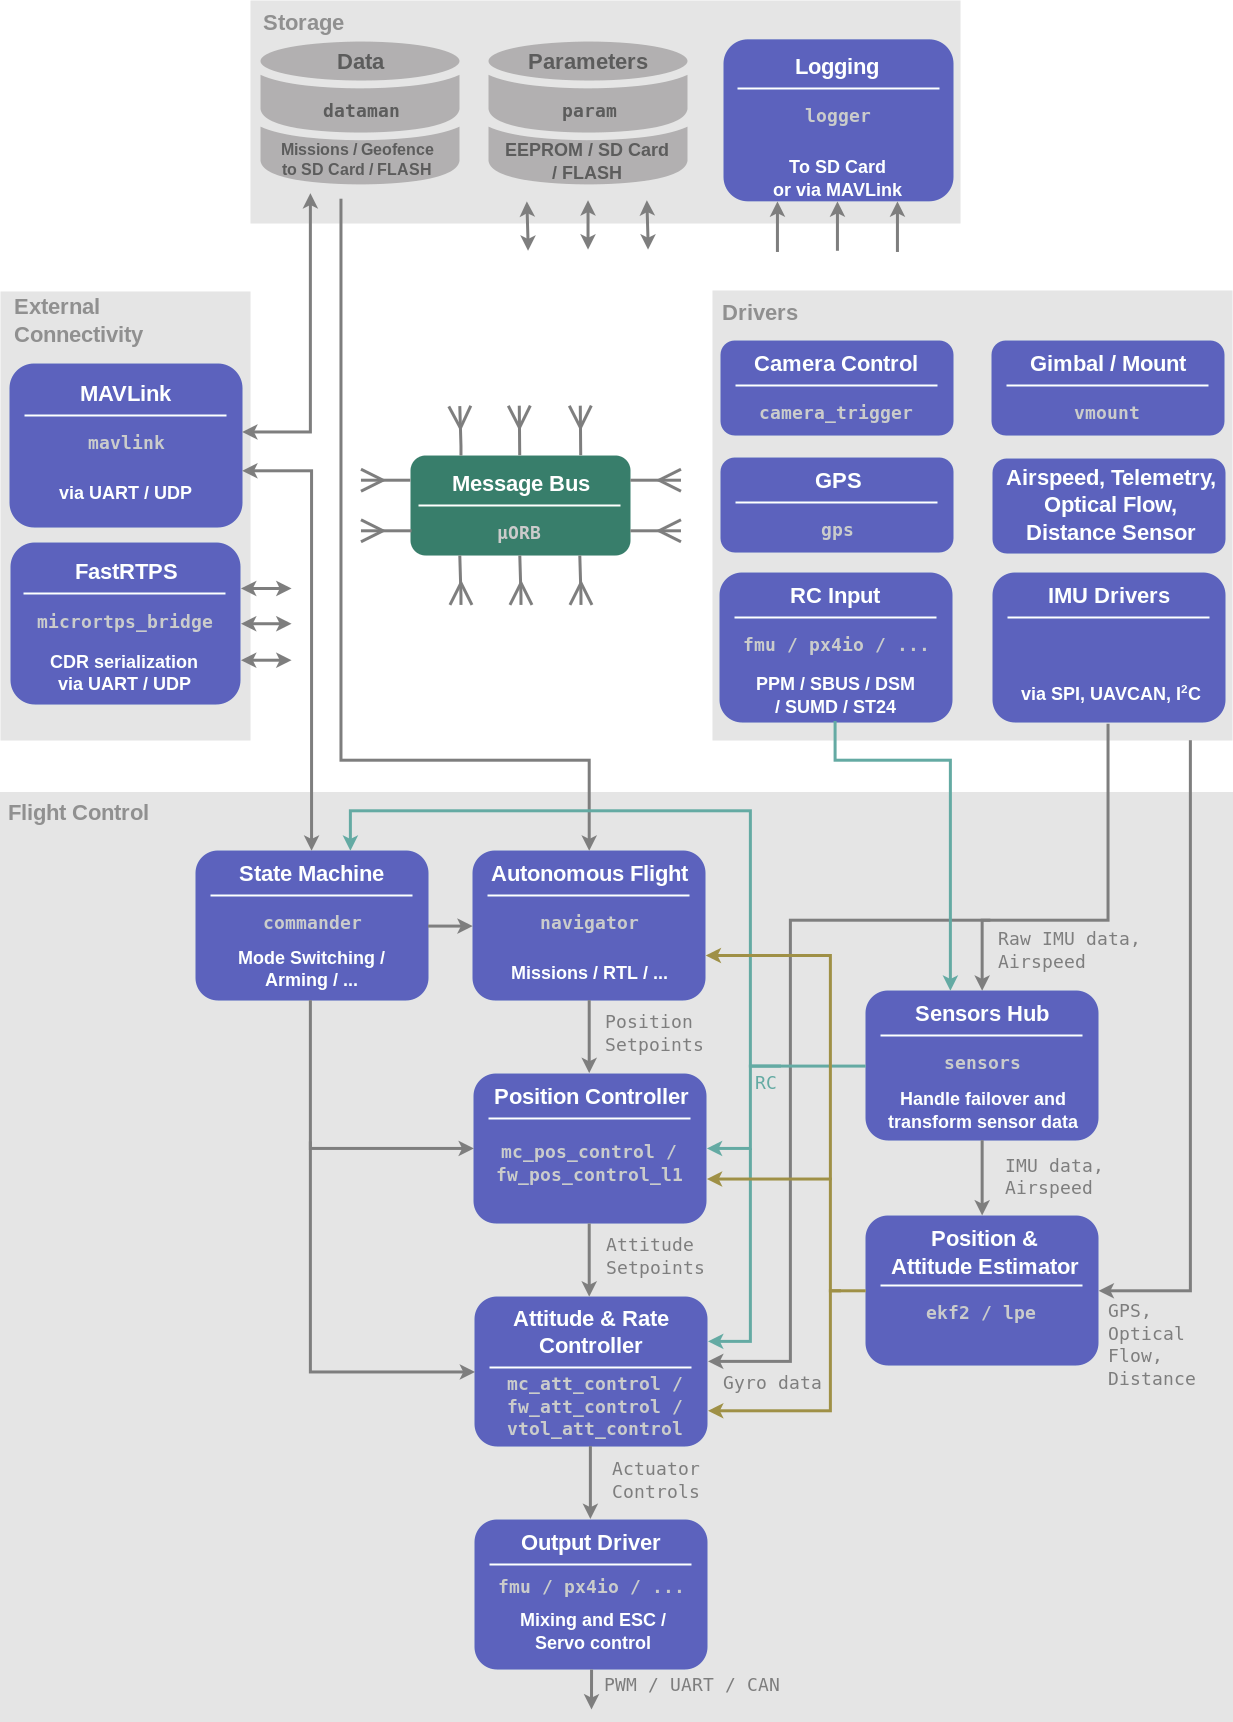
\includegraphics[width=0.8\textwidth]{DescrizioneAutopilota/Figure/PX4_Architecture}
	\caption{Architettura del codice di PX4 Autopilot, \cite{px4Guide}}
	\label{fig:px4.architettura}
\end{figure}
\subsubsection{Flight stack}
Il flight stack, mostrato in figura \ref{fig:px4.flightstack} è l'insieme di moduli che si occupano della stima dello stato del sistema e di tutti le funzionalità per il controllo,la guida e la navigazione. Esiste anche un modulo per interfacciarsi con il volo manuale attraverso radiocomando.
	\begin{figure}[ht]
	\centering
	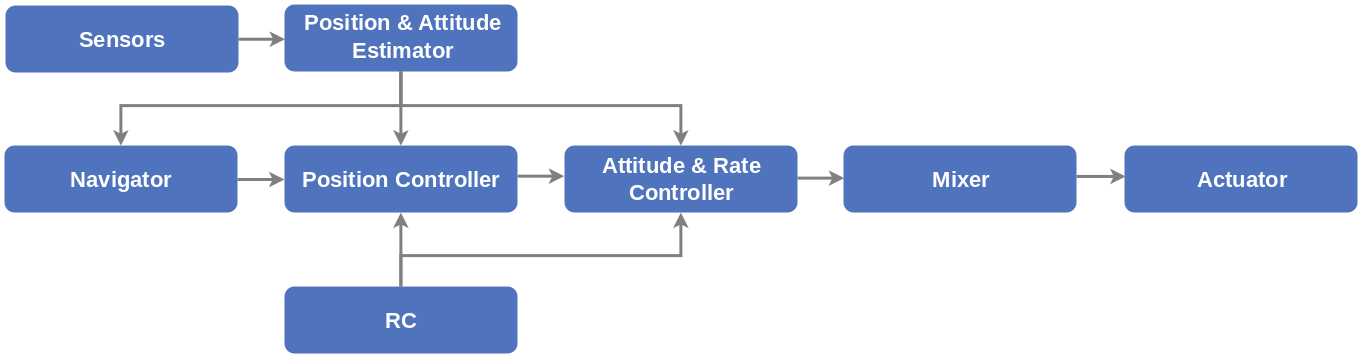
\includegraphics[width=1\textwidth]{DescrizioneAutopilota/Figure/PX4_High-Level_Flight-Stack}
	\caption{Architettura del flight stack di PX4, \cite{px4Guide}}
	\label{fig:px4.flightstack}
\end{figure}
\paragraph{Estimator}
L'estimator è il modulo che prendendo i dati da uno o più sensori determina lo stato attuale del velivolo. E' possibile selezionare diversi tipi di estimato, quello selezionato in questo caso è uno stimatore con filtro di Kalman.
\paragraph{Controller}
Si occupa di prendere in input i vari punti della pianificazione e confrontarli con lo stato attuale determinato dell'estimator. In questo modo vengono determinati i segnali di comando di output che saranno poi elaborati dal mixer. Questa funzionalità è implementata da più moduli, suddividendo la dinamica lenta e la dinamica veloce del drone. Verrà disabilitata la sua funzionalità per sostituirla con l'applicazione sviluppata su Simulink.
\paragraph{Mixer}
Il mixer si occupa di tradurre i segnali del comandi normalizzati di rollio, imbardata, beccheggio e manetta, da consegnare all'hardware che genera gli impulsi pwm utilizzati per il controllo del motore.
\subsubsection{Middleware}
Questo insieme di moduli si occupa invece di tutte le comunicazioni interne tra processi e tra PX4 e il mondo esterno. \'E composta principalmente dai driver per i sensori, i canali di comunicazione verso l'esterno e il bus di trasmissione di messaggi attraverso $\micro$ORB e MAVLink, \cite{MAVLink}. In questo contesto ricade anche  la connessione con un simulatore per testare il codice generato nelle varie fasi di validazione.
\subsection{Strumenti per lo sviluppo del codice}
Il sistema operativo utilizzato per lo sviluppo è Ubuntu 18.04.5 LTS, nella quale è stato installato MATLAB 2020a. Viene inoltre installato il tool "Embeded Coder Support Package for PX4 Autopilots", seguendo la guida, \cite{PX4MATLAB}. La versione di Ubuntu  installata però non è pienamente compatibile in quanto non è presente di default il software necessario al lancio delle simulazioni da parte di Simulink, ovvero "xterm", che va installato manualmente. La versione di PX4 utilizzata è quella prevista dalla guida \cite{PX4MATLAB}, ovvero la versione "1.8.0". Risulta inoltre necessario installare anche la versione di Java 8 e ROS-Melodic contenente il software Gazebo.

L'intero codice del firmware PX4 viene messo a disposizione attraverso la piattaforma github, \cite{PX4-FIRMWAREGIT}. Il progetto contiene all'interno le toolchain necessarie per compilare il sistema nei vari sistemi operativi. Agendo sulle varie possibili configurazioni di compilazione è possibile modificare e aggiunge delle funzionalità. Modificando le impostazioni di compilazione si può generare il programma finale da caricare ed eseguire sull'autopilota.
Sono presenti anche delle configurazioni per effettuare l'analisi e la verifica del codice generato attraverso l'utilizzo di un ambiente simulato. I simulatori che presentano una configurazione di base sono : Gazebo, jMAVSim , AirSim, Xplane. Per quanto riguarda questa tesi, verrà utilizzato il software Gazebo sfruttando parzialmente il codice già presente e adottando alcune modifiche. Nulla vieta comunque di poter collegare un simulatore diverso attraverso la creazione di un interfaccia dati con il firmware. Infatti, la connessione viene effettuata attraverso UDP o seriale, utilizzando su essa il protocollo MAVLink.

Per la generazione del codice sorgente da implementare nel firmware PX4, si fa utilizzo delle funzionalità aggiunte a MATLAB/Simulink dal tool "Embeded Coder Support Package for PX4 Autopilots", \cite{PX4MATLAB}. Dopo l'installazione di questo pacchetto vengono aggiunti alla libreria standard di Simulink, alcuni blocchetti utili all'interfacciamento con le restanti parti del firmware di PX4. Attraverso l'utilizzo di messaggi $\micro$ORB avvengono infatti le comunicazioni con i moduli eseguiti parallelamente alla configurazione del firmware: stimatore, sensori, attuatori ecc.

Nella creazione del modello in Simulink, si è tenuto conto del fatto che i dati necessari al controllo, venissero prelevati dallo stimatore di default di PX4, a differenza del lavoro svolto precedentemente in \cite{DesTestCarm}, nella quale si sono implementati le funzioni dei sensori e uno stimatore specifico.

Attraverso l'uso dei messaggi passati dal Firmware a Simulink quindi si sono implementati i controllori come spiegato in dettaglio nel capilo precedente. Nella Figura (\ref{fig:in}), viene mostrato l'implementazione su simulink necessaria a leggere lo stato del drone.

\begin{figure}
	\centering
	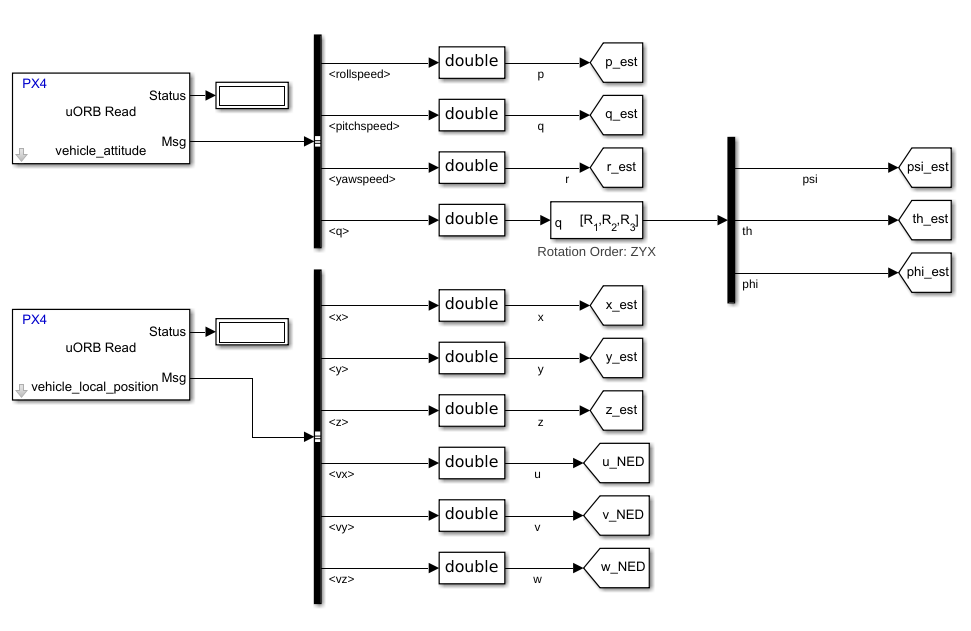
\includegraphics[width=0.6\textwidth]{DescrizioneAutopilota/Figure/IN}
	\caption{Interfaccia di input del modulo di controllo implementato su Simulink}
	\label{fig:in}
\end{figure}

Analogamente avviene il collegamento in output del sistema di controllo con l'apposito modulo della libreria, Figura (\ref{fig:out}).

\begin{figure}
	\centering
	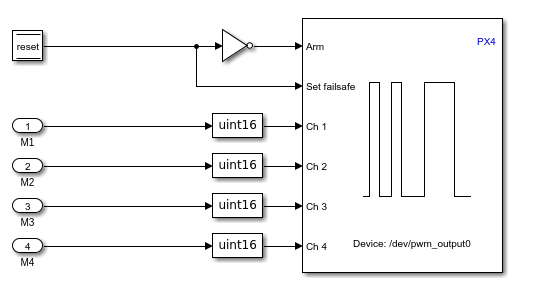
\includegraphics[width=0.5\textwidth]{DescrizioneAutopilota/Figure/OUT}
	\caption{Interfaccia di output del modulo di controllo implementato su Simulink}
	\label{fig:out}
\end{figure}

Utilizzando quindi questi moduli in input e output, il Coder è in grado generare il codice sorgente, incapsularlo in un modulo di PX4 e compilarlo. Da questo si ottiene quindi un file eseguibile con il sistema PX4 compilato e integrato in esso il controllo implementato. 

Nativamente il tool di Simulink sopracitato non permette l'utilizzo dell'ambiente Gazebo, ma solamente il simulatore jMavSim. Per questo è stato studiato il processo di lancio della simulazione integrato nel tool e la documentazione sui collegamenti tra il firmware PX4 e Gazebo nelle simulazioni SIL effettuate senza utilizzare Simulink. Attraverso la scrittura di uno script, presente in appendice, si è superata questa limitazione, rendendo possibile l'utilizzo di Gazebo per effettuare le simulazioni SIL. In Figura (\ref{fig:ig:INTERSIL}), viene mostrata la configurazione utilizzata per effettuare le simulazioni SIL. Come è possibile osservare nel caso si compili il codice per effettuare SIL, viene compilato all'interno del firmware un modulo che ha lo scopo specifico di interfacciare il simulatore con il Firmware. Il controllore utilizzato è integrato come modulo all'interno del firmware stesso.

\begin{figure}[!h]
	\centering
	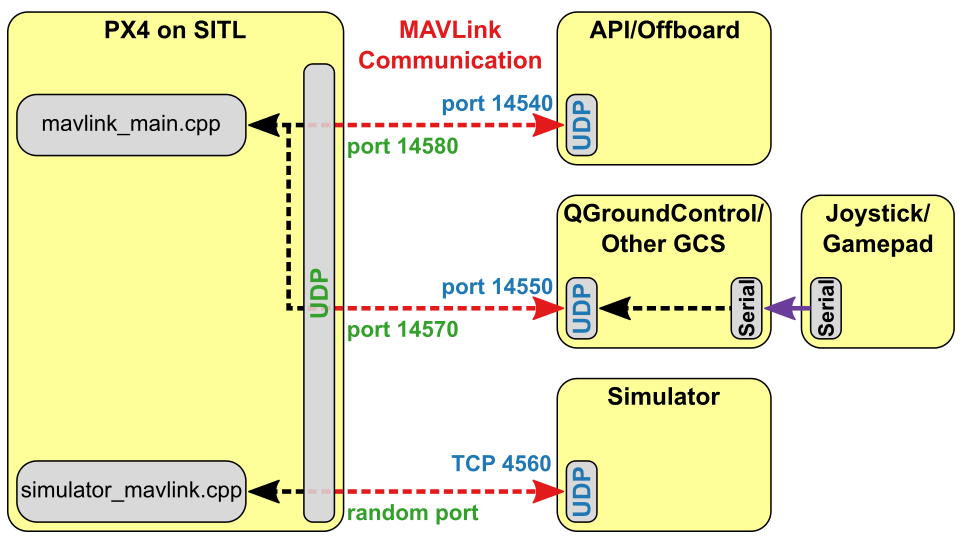
\includegraphics[width=0.5\textwidth]{DescrizioneAutopilota/Figure/INTERSIL}
	\caption{Configurazione per effettuare le simulazioni SIL}
	\label{fig:ig:INTERSIL}
\end{figure}


